\documentclass[journal,twoside,web]{ieeecolor}
\usepackage{generic}
\usepackage{cite}
\usepackage{amsmath,amssymb,amsfonts}
\usepackage{algorithm}
\usepackage{algorithmic}
\usepackage{graphicx}
\usepackage{textcomp}
\makeatletter
\def\BState{\State\hskip-\ALG@thistlm}
\makeatother

\def\BibTeX{{\rm B\kern-.05em{\sc i\kern-.025em b}\kern-.08em
    T\kern-.1667em\lower.7ex\hbox{E}\kern-.125emX}}
\markboth{\journalname, Project CARP, 11/24/2017}
{FANG Yidong, An Evolutionary Algorithm with Local Search for the Capacitated Arc Routing Problem}
\begin{document}
\title{An Evolutionary Algorithm with Local Search for the Capacitated Arc Routing Problem}
\author{FANG Yidong, Student No.11510493 \IEEEmembership{CSE, Southern University of Science and Technology}
}

\maketitle

\begin{abstract}
The capacitated arc routing problem (CARP) is a difficult vehicle routing problem where, given an undirected graph, the objective is to minimise the total cost of all vehicle tours that serve all required edges under vehicle capacity constraints. In this report, an evolutionary algorithm with local search is implemented based on Python to solve this problem. The algorithm applies the evolutionary mechanism to construct the whole framework, using two special heuristic initializing algorithm, which is random path scanning and augment merge, and the special local search for routing problems.
\end{abstract}

\begin{IEEEkeywords}
capacitated arc routing problem;
evolutionary algorithm;
local search;
order crossover;
path scanning;
augment merge;
\end{IEEEkeywords}

\section{Introduction}
\label{sec:introduction}
\IEEEPARstart{T}{he} capacitated arc routing problem (CARP) may be described as follows: consider an undirected connected graph $G=(V,E)$, with a vertex set $V$ and edge set $E$ and a set of required edges $R \subseteq E$. A fleet of identical vehicles, each of capacity $Q$, is based at a designated depot vertex. Each edge of the graph $(v_i ,v_j)$ incurs a cost $c_{ij}$ whenever a vehicle travels over it or services a required edge.When a vehicle travels over an edge without servicing it, this is referred to as deadheading. Each required edge of the graph $(v_i ,v_j)$ has a demand $q_{ij}$ associated with it. A vehicle route must start and finish at the designated depot vertex and the total demand serviced on the route must not exceed the capacity of the vehicle, $Q$. The objective of the CARP is to find a minimum cost set of vehicle routes where each required edge is serviced on one of the routes. The problem is proposed by Golden and Wong in 1981\cite{Golden1981}.
\par
In the instances tested, the objective is to minimise the total cost incurred on the routes and does not include any
costs relating to the number of routes or vehicles required.

\section{Evolutionary Algorithm}
%%% citation
The memetic algorithm introduced by Moscato (1989)\cite{Moscato1989}, also known as hybrid genetic algorithm or genetic local search, is a combination of a population-based global search GA and an individual-based local search. Several characters of our are: (1) An order crossover method is used to keep the balance of exploration and exploitation abilities; (2) the child of crossover will have a probability to go into a local search for better local optimal result; (3) one chromosome $P_r$ is selected in the parent population using binary tournament replacement, described in Algorithm \ref{algorithm:framwork}, and it is replaced by one child $C$ if the child $C$ is not a clone of any other chromosome than $P_r$ in the parent population, else a simple mutation is implemented on the child $C$ to diversify the population; (4) The algorithm will restart to increase the diversity of the population after a certain time of iteration. 
\par
The whole algorithm framework is showin in Algorithm \ref{algorithm:framwork}.
\begin{algorithm}
\caption{Main framework of the Algorithm}
\label{algorithm:framwork}
\begin{algorithmic} [1]

\STATE \textbf{Initialize} $ps$ individuals in the population $P$, in which $idv_0$ is generated by Augment Merge, and $idv_1,idv_2,...,idv_19$ is generated by Random Path Scanning.
\STATE $bestSoFar\leftarrow None$
\REPEAT
\REPEAT
\STATE $p_a, p_b \leftarrow$ randomSelect($P$)
\STATE $child1, child2 \leftarrow$ OrderCrossover($p_a,p_b$)
\STATE $newidv\leftarrow$ randomSelect($child1, child2$)
\STATE $rnd \leftarrow$ random number from 0 to 1
\IF{$rnd\leq $ Mutation rate $p_m $}
\STATE $newidv$ = localSearch($newidv$)
\ENDIF
\IF{Fitness($newidv$) $<max$\{Fitness($p_a$), Fitness($p_b$)$\}$}
\IF{Fitness($newidv$) $<$ Fitness($bestSoFar$)}
\STATE $bestSoFar\leftarrow newidv$
\ENDIF
\STATE $P_r\leftarrow$ parent with larger cost
\IF{$P_r\neq newidv$}
\STATE $P_r\leftarrow newidv$ 
\ELSE 
\STATE $newidv\leftarrow$ simpleMutation($newidv$)
\STATE $P_r\leftarrow newidv$ 
\ENDIF
\ENDIF
\UNTIL{$k$ max iteration number}
\UNTIL{time $t$ is very closed to the limited time}
\end{algorithmic}
\end{algorithm}
\subsection{Initial Solution Deriving}
\subsubsection{Path Scanning}
%%% citation
This method is based on the procedure proposed by Golden et al.\cite{Golden1983}. Each route is extended by one required edge at each step using a variety of selection rules. Each route starts at the depot vertex. Let $S$ be the set of required edges closest to the end of the current route that are not yet served and do not exceed the capacity of the current route. If $S$ is empty then complete the current route using the shortest deadheading path from the end of the current route to the depot vertex and start a new route. If $S$ is not empty, exclude from $S$ any edges that would close the route unless that would make S empty. Select a required edge in S to be the next edge in the route to be serviced according to the current rule and extend the current route to the vertex at the end of the selected edge. Five rules are used to determine the next required edge, $e$, in the route to be serviced: (1) minimise the distance to to the end of the current route; (2) maximise the ratio $d_{ij}$/$c_{ij}$, where $d_{ij}$ and $c_{ij}$ are, respectively, the demand and the cost of $(v_i ,v_j)$; (3) minimise this ratio; (4) minimise the return cost; (5) use rule 1 if the vehicle is less than halffull, else use rule 4;  Each criterion gives rise to one solution and the best of the five is chosen.
\par
In our implementation we set the rule 1 as the highest priority. Then, if the two required edge have the same distance, we will randomly choose one rule to break the tie. The details are shown in Algorithm \ref{algorithm:path-scanning}.
\begin{algorithm}
\caption{Random Path-Scanning for one priority rule}
\label{algorithm:path-scanning}
\begin{algorithmic} [1]
\STATE $k \leftarrow 0$
\STATE copy all required arcs in a list $free$
\REPEAT
\STATE $k\leftarrow k+1; R_k \leftarrow \o; load(k), cost(k)\leftarrow 0; i\leftarrow 1$
\REPEAT
\STATE $\overline{d} \leftarrow \infty$
\FOR{\textbf{each} $u \in free | load(k)+1_u \leq Q$}
\IF {$d_{\underline{i},beg(u)}<\overline{d}$}
\STATE $\overline{d} \leftarrow d_{\underline{i},beg(u)}$
\STATE $\overline{u} \leftarrow u$
\ELSIF{$d_{\underline{i},beg(u)}=\overline{d}$and $better(u,\overline{u},rule)$}
\STATE $\overline{u} \leftarrow u$
\ENDIF
\ENDFOR
\STATE add $\overline{u}$ at the end of route $R_k$
\STATE remove arc $\overline{u}$ and its ooposite $\overline{u}+m$ from $free$
\STATE $load(k)\leftarrow load(k)+\underline{q}_{\overline{u}}$
\STATE $cost(k)\leftarrow cost(k) + \overline{d} + \underline{c}_{\overline{u}}$
\UNTIL{$free = \o $ or $(\overline{d}=\infty)$}
\STATE $cost(k) \leftarrow cost(k) + d_{i1}$
\UNTIL{$free = \o$}
\end{algorithmic}
\end{algorithm}
\subsubsection{Augment Merge}
%%% citation
Augment-Merge (AM), just sketched in 1981 by Golden and Wong \cite{Golden1981}, was detailed in 1983 by Golden, DeArmon, and Baker \cite{Golden1983}. It is inspired by the Clarke and Wright Heuristic (CWH) for the CVRP \cite{Clarke2012}. The heuristic builds first one direct trip for each
required edge. Then, a Merge phase is executed, in which each iteration considers each pair of routes and evaluates the saving if the two routes are merged (concatenated). There are four ways of merging two given routes, as each route can be reversed or not. The merger with the largest saving is executed, and this process is repeated until no merger is possible without violating vehicle capacity.
\par
Compared with CWH, a preliminary phase called Augment is added. The initial routes are sorted in nonincreasing order of costs. Recall that we represent a route as a list of required arcs (see introduction). Starting from the longest route, each route $R_k =( (i,j)), k = 1,2,...,t-1$, is compared with each shortest route $R_p$, $p = k + l,k + 2,...,t$ such that the sum of their loads fits vehicle capacity. If the unique edge serviced by $R_p$ lies on $SP_{1i}$ or $SP_{j1}$, it can be transferred in $R_k$ and $R_p$ can be replaced by an empty trip. The cost of $R_k$ does not change, but a saving equal to the cost of $R$ is incurred. The Augment phase can strongly reduce the total cost and the number of routes before starting the Merge phase. \par
This nontrivial heuristic is detailed in Algorithm 7.3 of book \textit{Arc Routing}\cite{Corberan2015}, where $F_k$ and $L_k$ denote the first and last node of route $R_k$. The Augment phase can be implemented in $O(nt^2)$, while the Merge phase is dominated by the sort line 24 in $O(t^2logt)$. The whole complexity is then $O(t^{2}(n+logt))$, or $O(m^2n)$ if all edges are required.

\subsection{Chromosomes structure and evaluation}
\label{sec:chromesome}
To describe the tasks clearly, each required edge is identified by being marked a task number instead of one pair of nodes. Each edge $u \in E$ has a tail (start node) $a(u)$, a head (end node) $b(u)$, and a traversing (deadheading) cost $tc(u)$. Each required edge (task) $u \in E_R$ has a demand $d(u)$, a serving cost $sc(u)$, and an inverse mark $inv(u)$. Task $inv(u)$ and $u$ have the same traversing demand, and serving costs. Note that each edge task $u\in E_R$ can be served in either direction, i.e., only one of task $u$ and $inv(u)$ is served. Inspired by Lacomme, Prins, and Ramdane-Cherif\cite{Lacomme2001}, our chromosome T is a permutation of t required edges (tasks), without route delimiters. Implicit shortest paths are between consecutive tasks. They can be viewed as a RPP or a giant tour.

\begin{figure}[!t]
\centerline{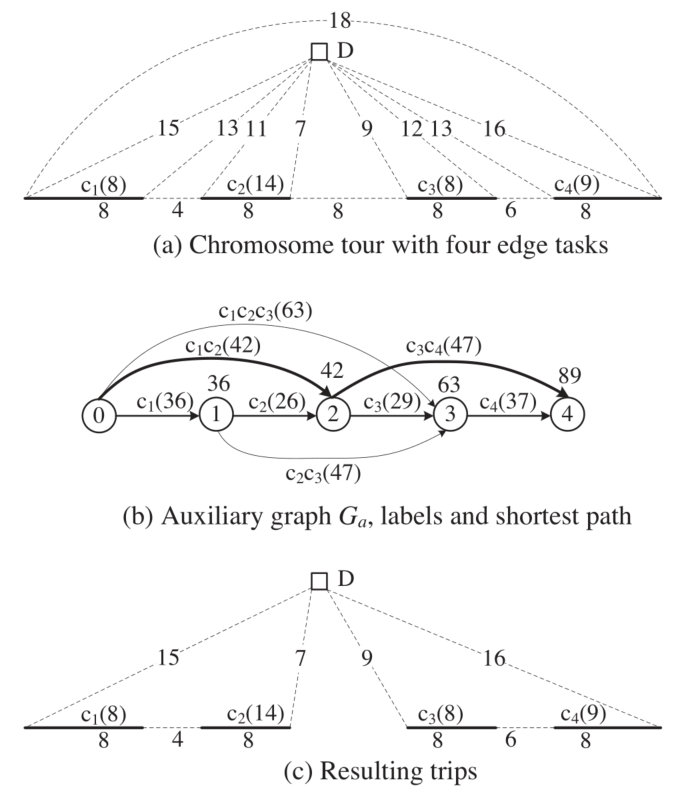
\includegraphics[width=\columnwidth]{chromesome.png}}
\caption{Example of Partition}
\label{chromesome}
\end{figure}

\par
% citation
Under this kind of chromosomes structure, the chromosome must be converted into a CARP solution by a partition (Ulusoy 1985)\cite{Ulusoy1985} procedure which corresponds to chromosome decoding and can evaluate the performance of each chromosome. The fitness is the total cost of this solution. Given a chromosome $T=(c_1, c_2,...,c_t)$ where $t$ corresponds to the number of tasks, the partition procedure works on an auxiliary directed acyclic graph $G_a=(X,Y,Z)$, where $X$ is a set of $t+1$ vertex indices from a dummy node $0$ to $t$. $Y$ is a set of arcs where one arc $(i,j)\in Y$ means that a trip serving tasks subsequence $c_{i+1}, c{i+2},...,c_j$ is feasible in terms of capacity, i.e., $load(i+1,j)\leq Q$ where loadði þ 1;jÞ is the load of the trip.
Z is the set of the weight of arcs where one weight z ij corresponds to the total cost of one vehicle to serve task subsequence $c_{i+1}, c{i+2},...,c_j$. The optimal partitioning of the chromosome $T$ corresponds to a shortest path from node $0$ to node $t$ in $G_a$. Thus, this problem is a shortest path problem (SPP), which can be solved in pseudo-poly-
nomial time based on Bellman’s algorithm.
Consider one example of vehicle capacity $Q=30$ and four edge tasks with their respective demands being 8, 14, 8, and 9. Figure \ref{chromesome}(a) shows the chromosome tour $T=(c_1, c_2,c_3,c_4)$ with demands in brackets. Thin dotted lines represent shortest paths between any two nodes, the numbers under $t=4$ tasks are the serving costs, and $D$ represents the depot. The partition procedure builds an auxiliary graph G a with t+1 nodes indexed from $0$ to $t$, as shown in Figure \ref{chromesome}(b). Arc $(0, 1)$ represents the trip $(0, c_1 , 0)$, where the first $0$ and the last $0$ correspond to the depot. A shortest path from node $0$ to node $t$ in $G_a$ (bold) indicates the optimal partitioning of $T$: two trips with total cost of $89$. The resulting CARP solu-
tion is the trip $(0, c_1 , c_2 , 0)$ with a cost of 42 the trip $(0, c_3 , c_4 , 0)$ with a cost of 47, as shown in Figure \ref{chromesome}(c).

\subsection{Reproduction Step and Extended OX Crossover}
The crossover operator is analogous to reproduction and biological crossover. In this more than one parent is selected and one or more off-springs are produced using the genetic material of the parents. In the algorithm, we apply the Davis’ Order Crossover (OX1). \par
\begin{figure}[!t]
\centerline{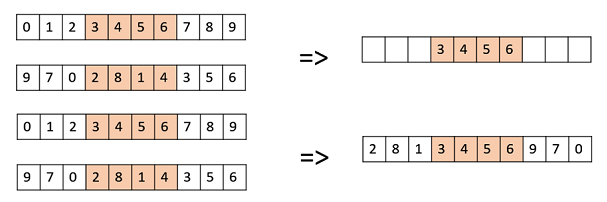
\includegraphics[width=\columnwidth]{ox.png}}
\caption{Illustration of the Order Crossover}
\label{ox}
\end{figure}
OX1 is used for permutation based crossovers with the intention of transmitting information about relative ordering to the off-springs. It works as follows, and the process is illustrated in Figure \ref{ox}.
\begin{itemize}
  \item Create two random crossover points in the parent and copy the segment between them from the first parent to the first offspring.
  \item Now, starting from the second crossover point in the second parent, copy the remaining unused numbers from the second parent to the first child, wrapping around the list.
  \item Repeat for the second child with the parent’s role reversed.
\end{itemize}
\par There exist a lot of other crossovers like Partially Mapped Crossover (PMX), Order based crossover (OX2), Shuffle Crossover, Ring Crossover, etc.
Parents are chosen by binary tournament selection. We first randomly select two solutions from the population. We then select from these two the least cost solution to be the first parent P1. This procedure is repeated to get the second parent P2. The two parents undergo an extended version of the classical order crossover (OX). The reproduction step ends by randomly keeping only one child C and by discarding the other. This policy works slightly better than keeping two children or the best one. \par
For two parents P1 and P2 of length t, the classical OX crossover draws two random subscripts $p$ and $q$ with $1\leq p \leq q \leq t$. To build child C1, it copies the string P1[p]-P1[q] into C1[p]-C1[q]. Finally, it scans P2 in a circular way from $q+1$ (mod t) and copies each element not yet taken to fill C1 circularly, starting from $q+1$ (mod t) too. The roles of P1 and P2 are exchanged to get the other child C2. OX must be
extended for the CARP and our data structure. Each chromosome contains all $t$ tasks,
but an edge can appear as one internal arc $u$ or as its inverse $inv(u)$. Therefore, when copying $u$ from a parent, we must check whether $u$ and $inv(u)$ are not already taken.
\subsection{Local Search as Mutation Operator}
We mutate with a fixed rate pm the child C produced by the crossover. The mutation
operator is a local search LS, giving a hybrid GA. It is clear nowadays that hybrid GAs
are better than Holland’s basic GA and can even outperform other metaheuristics.
Before applying LS, the child is converted into a set of trips, using steps 2-3 of
Ulusoy’s algorithm. Each iteration of LS scans in $O(t^2)$ all possible ways of moving a
task (in one trip or to another trip) and all possible permutations of two tasks (in one
trip or between two distinct trips). The collecting direction of an edge-task $u$ may be
inverted during this process, i.e. we try to reinsert $u$ or $inv(u)$. We also inspect two kinds of 2-opt moves by removing two shortest paths (possibly empty) $u-v$ and $x-y$, in the same trip or in distinct trips ($u$, $v$, $x$ and $y$ denote a task or the depot loop). We replace them by shortest paths $u-y$ and $v-x$ or by paths $u-x$ and $v-y$. 2-opt moves are not always possible in mixed networks because they may invert the trip order.\par
At each iteration, the first improving move is executed. The process is repeated
until no further saving can be found. Some trips may become empty and are removed
at the end. The child C is kept. A new chromosome S is rebuilt from the final trips (by
concatenating their tasks) and re-evaluated with step 2 of Ulusoy’s algorithm mentioned in section \ref{sec:chromesome}. Quite often, this slightly improves LS by shifting some trip limits.
The local search steps include:
\begin{itemize}
\item Flip one task a, i.e., replace a by inv(a) in its trip,
\item  Move one task a after another task or after the depot,
\item  Move two consecutive tasks a and b after another task or after the depot,
\item  Swap two tasks a and b,
\item  2-opt moves
\end{itemize}•
\section{Code Implementation}
In this project, all the code are implemented based on Python2, and none of external packages is used except numpy. The code are also written in an Objected-oriented way, which mainly contains classes for undirected graph, directed graph and the solver.
\subsection{Data Structures}
For the storage of the infomation for the edges and nodes, a class is defined, and most of the infomation is stored in the python multi-level dict structure, which can be defined and retrived in O(n) time. For the first and second level, we use the node numbers as keys and in the third level, the attribes like cost and demand are considered. For convenience, a set for storing the tasks is also defined for quick iteration over tasks.
\par At the same time, the Floyd-Warshall algorithm is implemented for the generating of all shortest paths between every two nodes. This algorithm is based on Dynamic Programming and the complexity is $O(|V|^3)$, where $|V|$ is denoted as the number of nodes in the graph.
\par In the main algorithm, servel data structures are used. The most important ones are the dict for storing the infomation for each individual in the population. The field of it is shown below:
\begin{itemize}
\item chromesome: list, a list of tasks without delimiters
\item partition: list of list, the route derived from chromesome with optimal delimiters, which can be get by the Ulusoy partition algorithm mentioned previously.
\item load: list, the load for each trip in the route, used for fast load calculation, which will be metioned in Section \ref{sec:tricky}.
\item cost: list, the cost for each trip in the route, similar usage to load's
\item fitness: int, the total cost of the solution.
\end{itemize}
\subsection{Multi-processing for Computing and Multi-threading for Controlling}
In our algorithm, the paralleling is only applied on the level of the whole algorithm, which means it just like running the same algorithm for a couple of time and the progrom put it on different processers. The number of computing processors can be adjusted in the main entrance file.\par
There are together two theads in the main process. One thread is used for timing and terminate the processors when the time is up while the other one is in charge of collecting the new solution from a queue where the computing processors are pushing the solutions in.
\subsection{Some Tricky Points: the Calculation During Local Search}
\label{sec:tricky}
During the development, it is found that because the complexity, the time cost during the local search is extremely large (It takes around 26 seconds for a solution in \textit{egl-s1-A.dat} to scan the inverse of each tasks in the solution). This is the evaluation Thus the complexity of the local search actully increased to $O(t^3)$.
A very usedful optimization proposed in our program is that we try to calculate the difference between original solution and the new solution, this significatly reduces the computation time to about 10\% of the original one.

\section{Computational Result}
Our experiment is taken on a VMWare-based virtual machine. The host of it is WINDOWS 10, with an Intel Core i7-6700 CPU and 8 GB memory. The CPU has 8 logical Processors and two of them is assigned to the virtual machine.\par
The algorithm is tested on servel standard instances given with the project files. And the results are listed in Table \ref{table:result}. Note that each average number is calculated by 6 runs with different random seeds.
\begin{table}
\caption{Computational result}
\label{table:result}
\setlength{\tabcolsep}{3pt}
\begin{tabular}{|p{40pt}|p{28pt}|p{28pt}|p{28pt}|p{28pt}|p{28pt}|p{30pt}|}
\hline
    Instance       & 10s\par Quality\par  Diff & 20s\par Quality\par Diff & 30s\par Quality \par Diff & 60s\par Quality\par Diff & 90s\par Quality\par Diff & Optimal \par Solution \\ \hline
       egl-e1-A-10 &    3960 \par 11.60\%  &    3843\par 8.32 \%  &    3794\par 6.95 \% &    3789 \par 6.80\%  &    3725\par 4.98\%   &    3548          \\ 
       egl-s1-A    &    6344 \par 26.42\% &    6273\par 25.00\%  &    6206\par 23.67\%  & 6020\par 19.79\%     &    5950\par 18.58\%  &    5018          \\ 
       gdb1        & 316 \par 0\%     & 316 \par 0\%    & 316 \par 0\%      & 316 \par 0\% & 316 \par 0\%    & 316      \\
       gdb3        & 281\par 2.08\%          & 277 \par 0.83\%            & 277  \par 0.83\% & 275\par 0\% & 275\par 0\% & 275               \\
       val1A       & 180 \par 4.13\%  & 180 \par 4.13\%   & 179 \par 3.22\% & 176 \par 1.65\% & 176 \par 1.65\%    & 173    \\
       val4A       & 444 \par 11.00\%     & 436  \par 8.89\% & 434 \par 8.61\%  & 431 \par 7.86\% & 426\par 6.43\%& 400    \\
       val7A       & 313 \par 12.19\%   & 305 \par 9.47\%   & 302 \par 8.24\%     & 297 \par 6.40\% & 297 \par 6.40\%  & 277     \\ \hline

\end{tabular}
\label{tab1}
\end{table}

\section{Result Analysis and Further Direction}
The result got by the algorithm is very good for the small-scal problem, while it is not so good for the problem with larger size, it is easy for the algorithm to sucked in a local optimal. This may be caused by the lack of variety in the population set. Some new initilization methods should be used to increse the variety of the population.\par
Also, the local search speed is still not very good compared to the large size of the population. There are two ways that may be effective to work around with the problem. First is try to parallelize the local search phase by local searching a lot of solution at the same time. Another point to  be improved is to continue scanning the same solution even when get a improvable point and update the solution in a global manner. This can avoid rescanning many repeated part of the same solution, but requires some sophisticated design of the local search algorithm.

\section{Conclusion}
In the evolutionary algorithm implemented by us, we combine several special methods to adjust to the conditions in the Capacitated Arc Routing Problem. Although the results can not still get very close to the best solutions compared to the state of art algorithm due to the limitation of time, a lot of useful algorithms and thoughts are learnt during the project.

 

\bibliographystyle{ieeetran}
\bibliography{reference}

\end{document}
